% !TeX spellcheck = it_IT
\newpage
\section{Ricerca locale}
La ricerca \emph{euristica} nello spazio di stati è troppo costosa ed è quindi necessario utilizzare metodi diversi. \\ Se prima gli algoritmi restituivano un cammino soluzione per raggiungere un goal, ora il goal è la soluzione stessa al problema. Gli algoritmi di ricerca locale sono adatti per problemi in cui:
\begin{itemize}
	\item La sequenza di azioni non è importante ma conta solo lo stato goal
	\item Tutti gli elementi della soluzioni sono nello stato ma alcuni vincoli sono violati
\end{itemize}
Questi algoritmi non sono sistematici e tengono traccia solo del nodo corrente spostandosi su quelli adiacenti. \\
Non tengono traccia dei cammini: rendono più efficiente l'occupazione della memoria e possono trovare soluzioni anche in spazi di stati molto grandi o infiniti.\\
Sono utili per risolvere problemi di \textbf{ottimizzazione}:
\begin{itemize}
	\item Stato migliore secondo una funzione obiettivo $f$
	\item Lo stato di costo minore (non il cammino)
\end{itemize}
Data la funzione euristica del costo dell'obiettivo
\begin{center}
	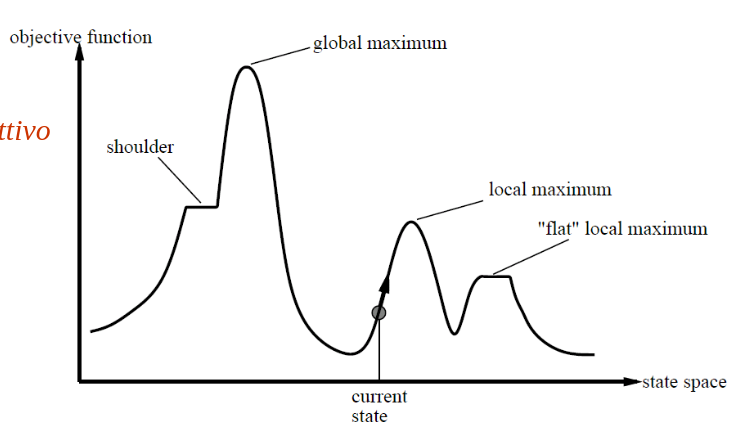
\includegraphics[scale=0.4]{ricerca_locale_spazio_stati.png}
\end{center}
uno stato ha una posizione sulla superficie e un'altezza che corrisponde al valore della valutazione della funzione obiettivo. Un algoritmo provoca movimento sulla superficie e l'obiettivo è raggiungere un punto in particolare (e.g. massimo locale).
\subsection{Hill climbing}
Sfrutta un principio di ricerca locale greedy dove vengono generati i successori e vengono valutati. Viene scelto un nodo che migliora lo stato attuale e scartati gli altri:
\begin{itemize}
	\item \textbf{Salita rapida} (o discesa): viene scelto il migliore
	\item \textbf{Stocastico}: scelta random
	\item \textbf{Prima scelta}: viene scelto il primo 
\end{itemize}
Se non ci sono successori che migliorano lo stato, l'algoritmo termina con fallimento.
\begin{lstlisting}[language=Python]
	def hill_climbing(problem):
		current = Node(problem.initial_state)
		while True:
			neighbors = [current.child_node(problem, action) for action in problem.actions(current.state)]
			if not neighbors: # se current non ha successori esci e restituisci current
				break
			# scegli il vicino con valore piu' alto (sulla funzione problem.value)
			neighbor = (sorted(neighbors,key = lambda x:problem.value(x), reverse = True))[0]
			if problem.value(neighbor) <= problem.value(current):
				break
			else:
				current = neighbor # (altrimenti, se vicino migliore, continua)
		return current
\end{lstlisting}
Non c'è frontiera a cui ritornare e si tiene un solo stato, quindi efficiente per la memoria. Il tempo necessario è variabile e dipende dal punto di partenza.\\

\subsubsection{8 regine}
Nel problema già descritto delle 8 regine, poniamo come funzione da minimizzare $h$ il numero di coppie di regine che si attaccano a vicenda. Bisogna minimizzare $h$.
Ogni regina può fare 7 mosse quindi abbiamo $7\cdot 8 = 56$ possibili stati successivi. Tra i migliori con lo stesso valore di $h$ si sceglie a caso.
\begin{example}[8 regine]
	Nel caso delle 8 regine:
	\begin{center}
		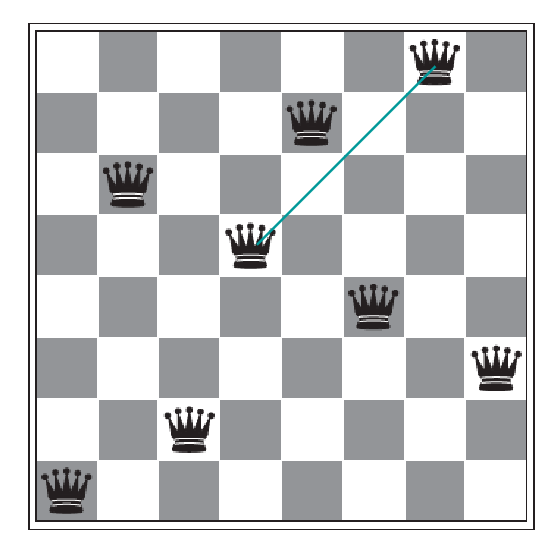
\includegraphics[scale=0.2]{8_regine_hill_climbing.png}
	\end{center}
\end{example}
Possiamo migliorare l'algoritmo in alcuni modi:
\begin{enumerate}
	\item Consentire un numero limitato di \textbf{mosse laterali}, ovvero l'algoritmo si ferma solo quando è peggiore la soluzione e non peggiore o uguale (sulle 8 regine $94\%$ di successo ma in media 21 passi)
	\item Hill-climbing \textbf{stocastico} (più lento ma soluzioni migliori)
	\item Hill-climbing \textbf{prima scelta}: genera mosse a caso fino a trovarne una migliore.
	\item Implementiamo un \textbf{riavvio casuale} che fa ripartire l'algoritmo da un punto a caso. Se la probabilità di successo è $p$, saranno necessarie $\frac{1}{p}$ iterazioni. Con molti minimi locali nella funzione obiettivo, $p$ si abbassa e aumentano il numero di volte in cui si blocca.
\end{enumerate}

\subsection{Tempra simulata}
Questo algoritmo combina hill-climbing con una scelta stocastica non totalmente casuale.\\
Ad ogni passo si sceglie un successore $n'$ a caso:
\begin{itemize}
	\item Se \textbf{migliora} lo stato corrente, viene espanso
	\item Se lo \textbf{peggiora} ($\Delta E = f(n')-f(n) \leq 0$) quel nodo viene scelto con probabilità $p=e^{\frac{\Delta E}{T}} \quad 0 \leq p \leq 1$.
\end{itemize}
Questo significa che $p$ è inversamente proporzionale al peggioramento. Con il progredire dell'algoritmo rende improbabili le mosse peggiorative.
\subsubsection{Scelta dei parametri}
I parametri sono il valore iniziale e il decremento di $T$. Il valore iniziale dovrebbe essere tale che per i valori medi di $\Delta E$ $p$ sia circa $0.5$.

\subsection{Local beam}
Dato l'algoritmo \emph{beam}, vengono salvati in memoria solo $k$ stati. Ad ogni passo si generano i successori di tutti i $k$ stati e:
\begin{itemize}
	\item Se si trova un goal, ci si ferma
	\item Altrimenti si prosegue con i $k$ migliori tra questi
\end{itemize}
\begin{note}
	È diverso da $k$ restart, in quanto non si riparte da $0$, e dal \emph{beam search} perché non si tengono tutti gli stati.
\end{note}
\subsubsection{Versione stocastica}
Si introduce un elemento di casualità: i $k$ successori vengono scelti con una probabilità maggiore per i migliori ma non tutti.
Introduciamo della terminologia:
\begin{itemize}
	\item \textbf{Organismo}: lo stato
	\item \textbf{Progenie}: i successori
	\item \textbf{Fitness}: il valore della funzione obiettivo
\end{itemize}

\subsubsection{Algoritmi genetici ed evolutivi}
Sono una variante della \emph{beam search stocastica} in cui gli stati successori sono ottenuti combinando due stati genitore invece che per evoluzione.
La \textbf{popolazione} iniziale è composta da $k$ \textbf{individui} generati casualmente e rappresentati come una stringa.
Gli individui sono valutati da una funzione di \textbf{fitness}. Vengono poi selezionati quelli per l'\textbf{accoppiamento} che danno vita alla generazione successiva in due modi:
\begin{itemize}
	\item \textbf{Crossover}: combinando il materiale genetico
	\item \textbf{Casuale}: con un meccanismo di mutazione genetica
\end{itemize}
Ogni generazione dovrebbe essere migliore della precedente.
\begin{example}[8 regine]
	Nel problema delle 8 regine abbiamo una popolazione di queste, dove le loro posizioni sono descritte da una stringa (ogni cifra è la riga in cui c'è la regina in quella colonna). La funzione di fitness è il numero di coppie di regine che non si attaccano.
	Per ogni coppia di combinazioni sulla scacchiera (scelta con la probabilità proporzionale alla fitness) viene scelto un punto di \textbf{crossing over} in maniera casuale e vengono generati due figli scambiandosi dei pezzi. Alla fine viene fatta una mutazione causale.
	\begin{center}
		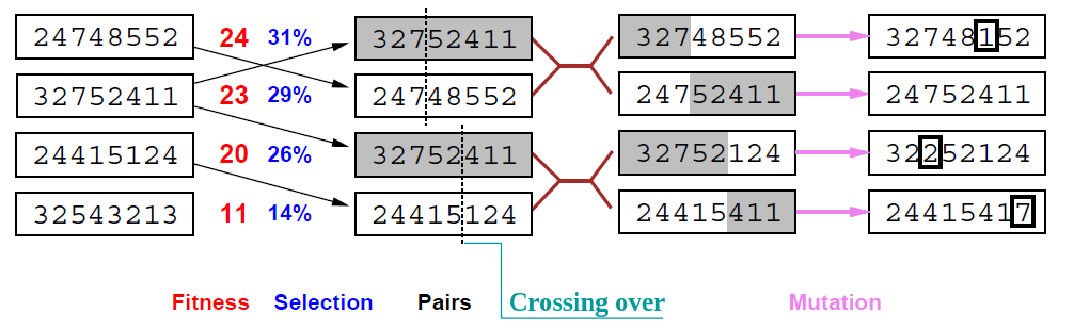
\includegraphics[scale=0.3]{alg_gen_ex.png}
	\end{center}
	\begin{center}
		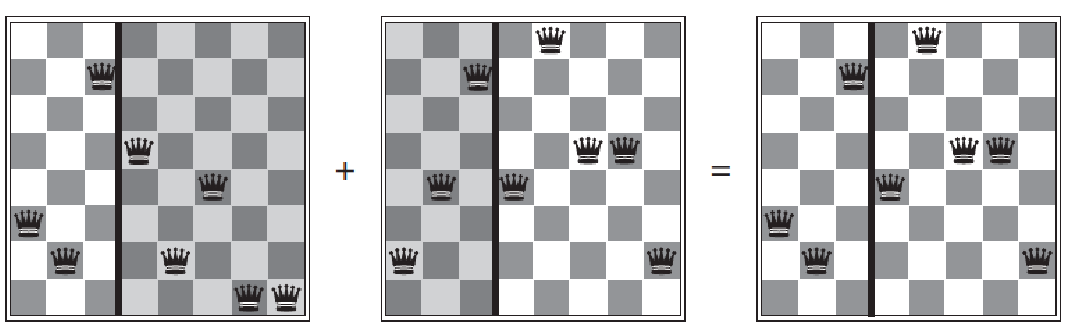
\includegraphics[scale=0.3]{alg_gen_ex_2.png}
	\end{center}
\end{example}
\noindent Questi algoritmi fanno parte del \textbf{Natural computer} e come vantaggi hanno:
\begin{itemize}
	\item Tendenza a salire della beam search stocastica
	\item Interscambio delle informazioni tra thread paralleli di ricerca in maniera indiretta
\end{itemize}
Questo tipo di algoritmi sono più efficaci se il problema ha componenti significative rappresentate in stringhe; è proprio la rappresentazione ad essere il punto critico.

\subsection{Spazi continui}
Lo stato è descritto da variabili \textbf{continue} in un vettore $x = x_1, \ldots, x_n$. Un esempio è lo spazio tridimensionale.\\
L'apparente difficoltà dovuta ai fattori di ramificazione infiniti è affrontata tramite strumenti matematici quali il \emph{gradiente}. Ad esempio l'\textbf{hill climbing iterativo} diventa:
\begin{equation*}
	x_{new} = x \pm \eta \nabla f(x)
\end{equation*}
sfruttando la direzione e lo spostamento che ci fornisce il gradiente invece di cercarlo tra gli infiniti successori.

\begin{example}
	Prendiamo la funzione $f(x)=x^2$ con derivata prima $f'(x)=2x$. Cerchiamo il minimo con
	\begin{equation*}
		x_{new}=x-\eta f'(x)
	\end{equation*}
	Partendo ad esempio da $x=2$ con $\eta=0.2$, otteniamo come primo risultato $x_{new} = 2-0.8=1.2$.
\end{example}

\subsection{Ambienti realistici}
A differenza dei problemi classici, il nostro ambiente è \textbf{parzialmente osservabile} e \textbf{non deterministico}. Qui le \textbf{percezioni} sono importanti in quanto restringono gli stati possibili e informano sull'effetto dell'azione.\\
L'agente deve elaborare una strategia con un piano di contingenza che tenga conto delle diverse eventualità.
\begin{example}[Aspirapolvere]
	\label{example:aspirapolvere}
	Un aspirapolvere imprevedibile ha due comportamenti:
	\begin{itemize}
		\item Se aspira in una stanza sporca la pulisce ma a volte pulisce anche una stanza adiacente
		\item Se aspira in una stanza pulita, a volte la sporca
	\end{itemize}
	La soluzione non è più una sequenza ma è un albero che gestisce il piano di di contingenza.
\end{example}

\subsubsection{Albero AND-OR}
È un albero che ha come nodi \emph{OR} le scelte dell'agente e come nodi \emph{AND} le diverse contingenze da considerare.
\begin{example}[Aspirapolvere]
	Nell'esempio \ref{example:aspirapolvere} l'albero sarebbe:
	\begin{center}
		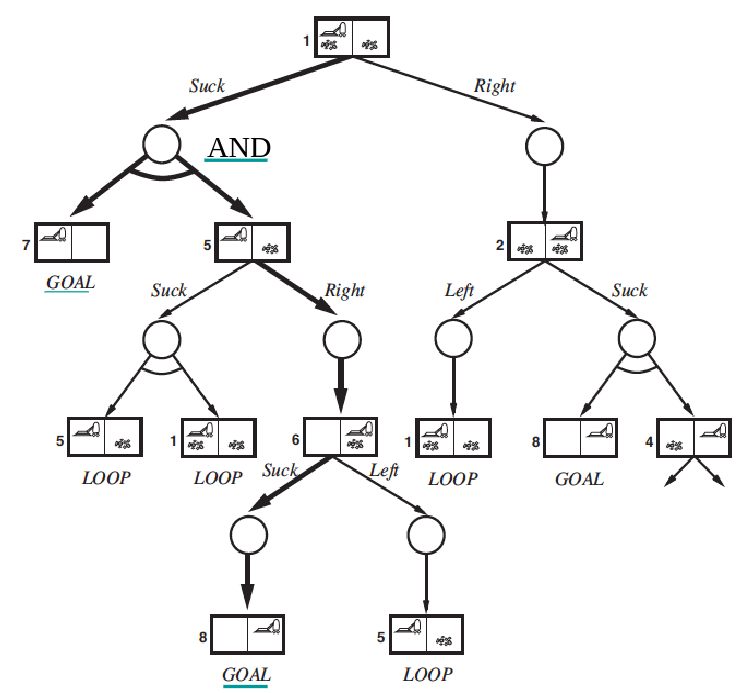
\includegraphics[scale=0.2]{example_aspirapolvere.png}
	\end{center}
\end{example}